\documentclass[]{article}

\usepackage{chronology}
\usepackage{float}
\usepackage{caption}
\usepackage{subcaption}
\usepackage{graphicx}
\usepackage{url}
\usepackage{amsmath}
\usepackage{amssymb}
\usepackage{amsthm}
\usepackage{tocloft}
\usepackage{cancel}
\usepackage{thmtools}
\usepackage[toc,nonumberlist,acronym]{glossaries}
\usepackage{glossaries-extra}
\usepackage{relsize}

\newcommand\numberthis{\addtocounter{equation}{1}\tag{\theequation}}
\newtheorem{defn}{Definition}
\newtheorem{thm}{Theorem}
\newtheorem{lemma}[thm]{Lemma}
\graphicspath{{figs/}}
\widowpenalty10000
\clubpenalty10000
\setcounter{tocdepth}{2}

\makeglossaries
%opening
\title{Computational Neuroscience Notes}
\author{Simon Crase}

\begin{document}
	
\newacronym{gls:EEG}{EEG\glsadd{gls:eeg}}{\Gls{gls:eeg}}

\newacronym{gls:fMRI}{fMRI\glsadd{gls:fmri}}{\Gls{gls:fmri}}

\newacronym{gls:MAP}{MAP\glsadd{gls:mpm}}{\Gls{gls:mpm}}

\newacronym{gls:ML}{ML\glsadd{gls:mlm}}{\Gls{gls:mlm}}

\newglossaryentry{gls:eeg}{
	name={Electroencephalography},
	description={a method to record an electrogram of the spontaneous electrical activity of the brain. The biosignals detected by EEG have been shown to represent the postsynaptic potentials of pyramidal neurons in the neocortex and allocortex.[1] It is typically non-invasive, with the EEG electrodes placed along the scalp (commonly called "scalp EEG") using the International 10-20 system, or variations of it. Electrocorticography, involving surgical placement of electrodes, is sometimes called "intracranial EEG". Clinical interpretation of EEG recordings is most often performed by visual inspection of the tracing or quantitative EEG analysis.\cite{enwiki:1128901597}}}

\newglossaryentry{gls:fmri}{
	name={Functional magnetic resonance imaging},
	description={Functional magnetic resonance imaging or functional MRI (fMRI) measures brain activity by detecting changes associated with blood flow. This technique relies on the fact that cerebral blood flow and neuronal activation are coupled. When an area of the brain is in use, blood flow to that region also increases\cite{enwiki:1124875371}}}

\newglossaryentry{gls:mlm}{
	name={maximum likelihood},
	description={Choose estimator $s^*$ to maximize $p[r\vert s]$
		}}
\newglossaryentry{gls:mpm}{
	name={maximum a posteriori},
	description={Choose estimator $s^*$ to maximize $p[s \vert r]$
}}

\newglossaryentry{gls:rf}{
	name={Receptive Field},
	description={Specific properties of a sensory stimulus that generate a strong response from the cell\cite{coursera2017cns}}}


\maketitle

\begin{abstract}
My notes from Computational Neuroscience course\cite{coursera2017cns}, which provides an introduction to basic computational methods for understanding what nervous systems do and for determining how they function.
\end{abstract}

\tableofcontents
\listoffigures
\section{Introduction and Basic Neurobiology}\label{sec:week1}

\subsection{Course Introduction}
\begin{figure}[H]
	\caption{Our Universes}
	\begin{subfigure}[t]{0.45\textwidth}
		\caption{According to Physicists}
		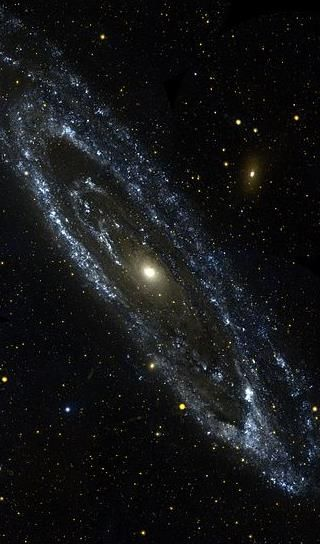
\includegraphics[width=\textwidth]{universe1}
	\end{subfigure}
	\begin{subfigure}[t]{0.45\textwidth}
		\caption{According to us}
		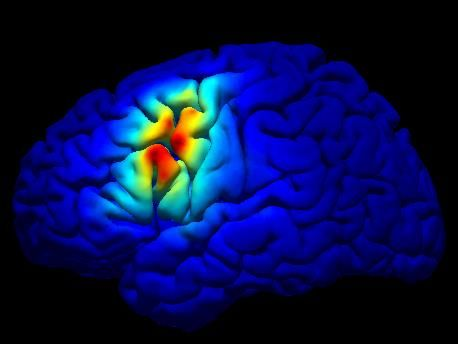
\includegraphics[width=\textwidth]{universe2}
	\end{subfigure}
\end{figure}
\subsubsection{Understanding the Brain using Computational Models}
\begin{itemize}
	\item Descriptive Models of the Brain
	\begin{itemize}
		\item How do neurons respond to external stimuli and how do we
		describe this quantitatively with a neural encoding model?
		\item How can we extract information from neurons (decoding)?
	\end{itemize}
    \item Mechanistic Models of Brain Cells and Networks
	\begin{itemize}
		\item     How can we simulate the behavior of a single neuron on a
	    computer?
	    \item How do we simulate a network of neurons?
	\end{itemize}
	\item  Interpretive (or Normative) Models of the Brain
	\begin{itemize}
		\item 	Why do brain circuits operate the way they do?
		\item What are the computational principles underlying their
		operation?
	\end{itemize}
\end{itemize}

\subsubsection{Course Goals: What you can expect to learn}
At the end of the course, you will be able to:
\begin{itemize}
	\item  Quantitatively describe what a biological neuron or
network of neurons is doing given experimental data
 \item Simulate on a computer the behavior of neurons and
networks
 \item Formulate computational principles underlying the
operation of neurons and networks in the brain
\end{itemize}

\subsection{Computational Neuroscience - Descriptive Models}

\subsubsection{Receptive Fields}
\begin{figure}[H]
	\caption[Responses of a Neuron in an Intact Cat Brain]{Responses of a Neuron in an Intact Cat Brain\cite{hubel1965receptive}}
	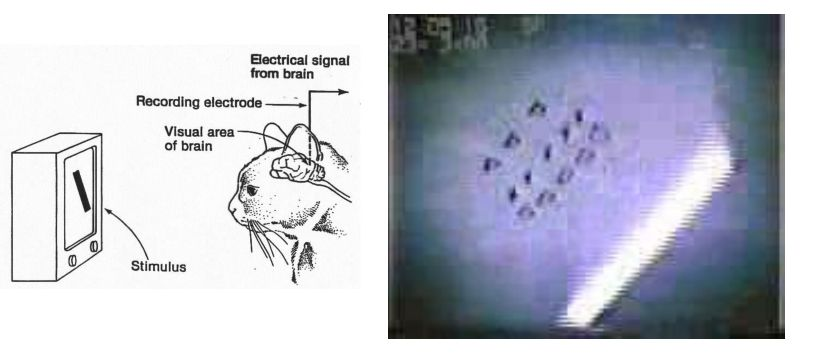
\includegraphics[width=\textwidth]{receptive-field-cat}
\end{figure}

\begin{figure}[H]
	\caption{Responses showing \gls{gls:rf}}
	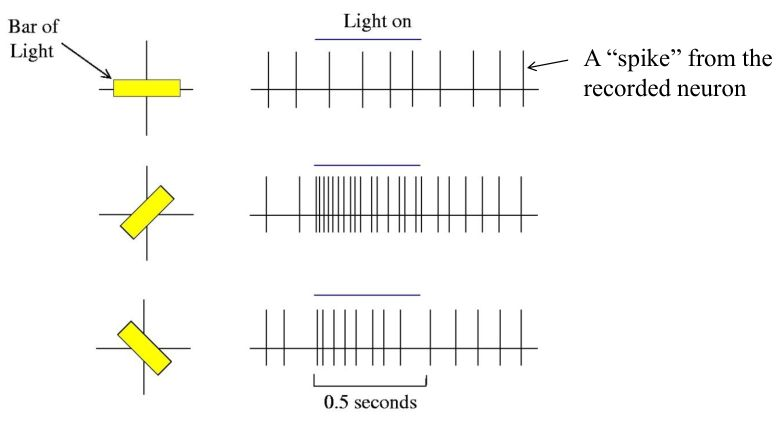
\includegraphics[width=\textwidth]{receptive-field-cat-bars}
\end{figure}

\subsubsection{Receptive Fields: a Descriptive Model}

\begin{figure}[H]
	\caption{Receptive Fields in the Retina}
	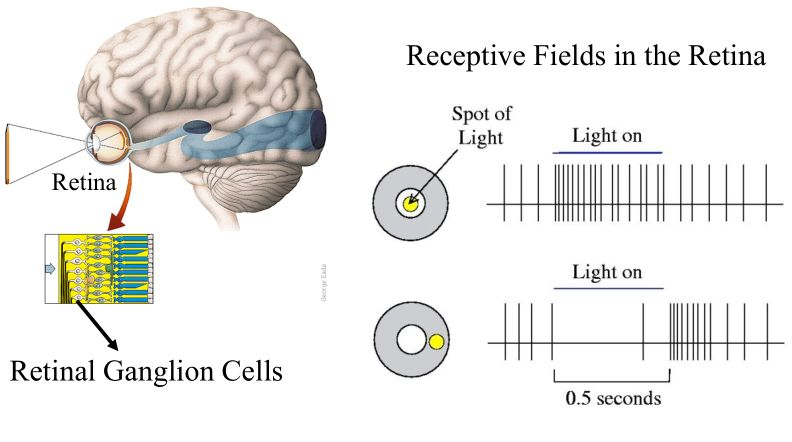
\includegraphics[width=0.8\textwidth]{receptive-fields-in-the-retina}
\end{figure}

\begin{figure}[H]
	\caption{Centre Surround Receptive Fields}
	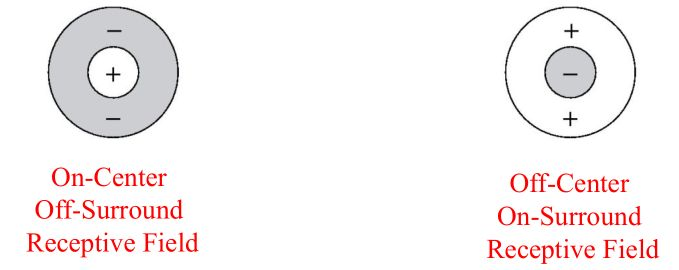
\includegraphics[width=0.8\textwidth]{center-surround}
\end{figure}

\begin{figure}[H]
	\caption{Cortical Receptive Fields}
	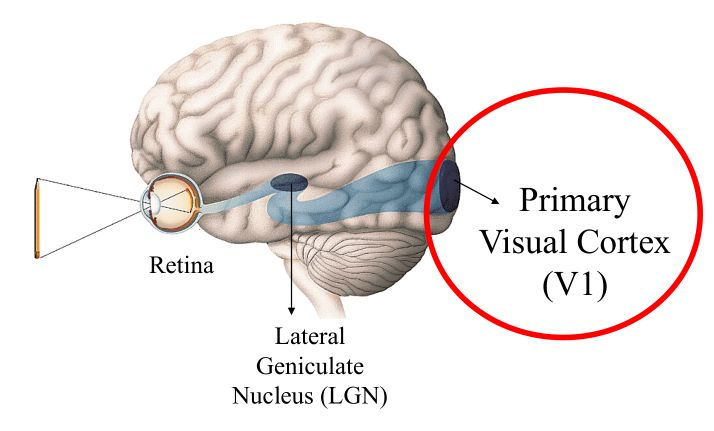
\includegraphics[width=\textwidth]{CorticalReceptive Fields}
\end{figure}

\begin{figure}[H]
	\caption{Oriented receptive field of a neuron in primary visual cortex (V1)}
	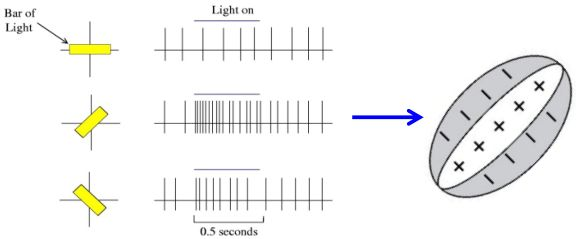
\includegraphics[width=\textwidth]{orientation-preference}
\end{figure}

\begin{figure}[H]
	\caption[How are these oriented receptive fields obtained?]{How are these oriented receptive fields obtained from center-surround receptive fields?}\label{fig:rf-shape}
	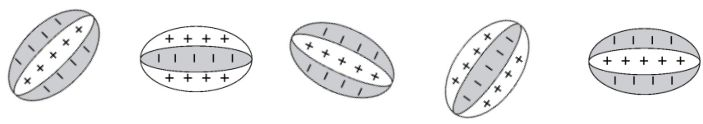
\includegraphics[width=\textwidth]{orientation-preference2}
\end{figure}

\subsection{Computational Neuroscience Mechanistic and Interpretive Models}


\begin{figure}[H]
	\caption[Receptive Fields: a Mechanistic Model]{Receptive Fields: a Mechanistic Model}
	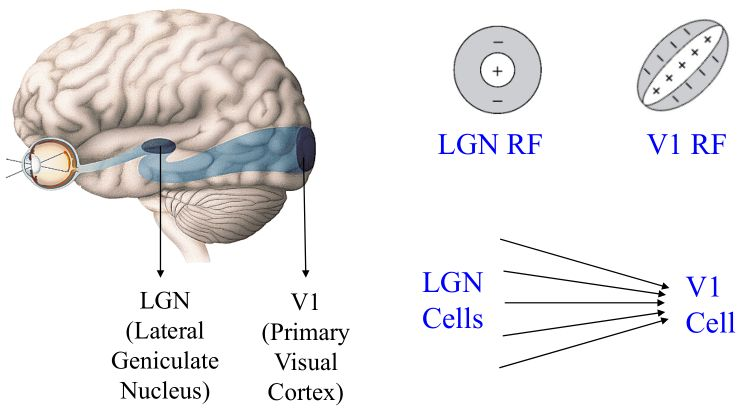
\includegraphics[width=0.9\textwidth]{mech-rf}
\end{figure}

\begin{figure}[H]
	\caption[Model suggested by Hubel \& Wiesel in the 	1960s]{Model suggested by 	Hubel \& Wiesel in the 	1960s: V1 RFs are 	created from converging
		LGN inputs. Center-surround LGN RFs are displaced along
		preferred orientation of V1 cell This simple model is still controversial!}
	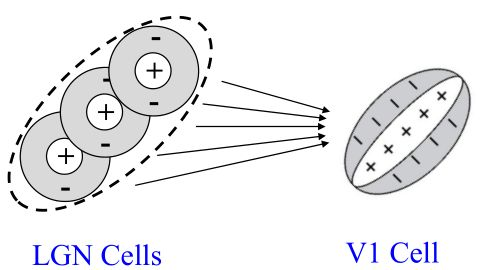
\includegraphics[width=0.9\textwidth]{mech-rf-v1}
\end{figure}

\subsubsection{Receptive Fields: an Interpretive Model}
Why are receptive fields in V1 shaped as in Figure \ref{fig:rf-shape}?

\begin{figure}[H]
	\caption[Efficient Coding Hypothesis]{Efficient Coding Hypothesis: suppose the
		goal is to represent images as faithfully and efficiently as possible using neurons with receptive fields $RF_1, RF_2$, etc}
	\begin{subfigure}[t]{0.2\textwidth}
		\caption{$RF_1$}
		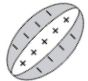
\includegraphics[width=0.7\textwidth]{rf1}
	\end{subfigure}
	\begin{subfigure}[t]{0.2\textwidth}
		\caption{$RF_2$}
		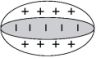
\includegraphics[width=\textwidth]{rf2}
	\end{subfigure}
	\begin{subfigure}[t]{0.2\textwidth}
		\caption{$RF_3$}
		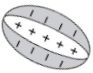
\includegraphics[width=\textwidth]{rf3}
	\end{subfigure}
	\begin{subfigure}[t]{0.2\textwidth}
		\caption{$RF_4$}
		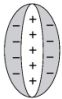
\includegraphics[width=0.5\textwidth]{rf4}
	\end{subfigure}
\end{figure}

Given image $I$, we can reconstruct it using neural responses $\{r_i\}$.
\begin{align*}
	\hat{I} =& \sum RF_i r_i
\end{align*}

What are the $RF_i$ that minimize the total squared pixelwise errors between $I$ and $\hat{I}$ and are as independent as possible?

\begin{figure}[H]
	\begin{center}
		\caption[Interpretive Model of Receptive Fields]{Interpretive Model of Receptive Fields: start out with random $RF_i$ and run your efficient coding algorithm on natural image patches}
		\begin{subfigure}[t]{0.9\textwidth}
			\begin{center}
				\caption{Natural Images}
				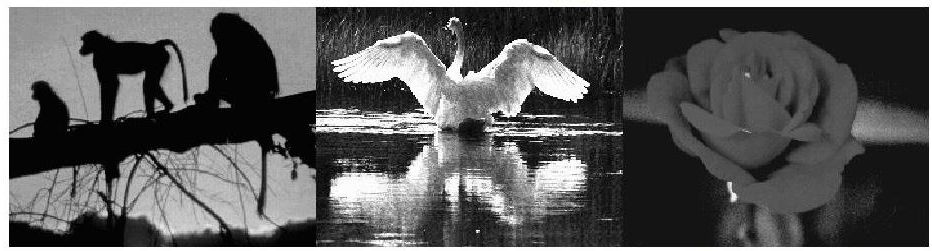
\includegraphics[width=0.7\textwidth]{natural-image}
			\end{center}
		\end{subfigure}
		\begin{subfigure}[t]{\textwidth}
			\caption{Receptive Fields from Natural Images}
			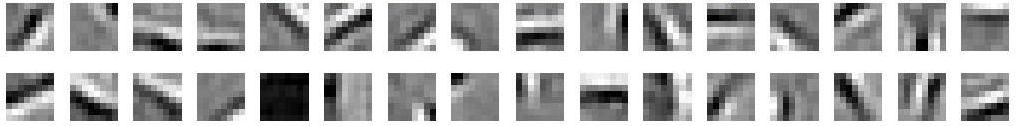
\includegraphics[width=\textwidth]{rf-natural}
		\end{subfigure}
		\begin{subfigure}[t]{\textwidth}
			\caption{Receptive Fields from V1, after Figure \ref{fig:rf-shape}}
			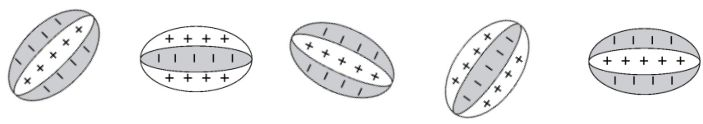
\includegraphics[width=\textwidth]{orientation-preference2}
		\end{subfigure}
	\end{center}
\end{figure}

 The brain may be trying to find faithful and efficient representations of an animal’s natural environment\cite{olshausen1997sparse,bell1997independent,rao1999predictive}

\subsection{The Electrical Personality of Neurons}

The neuron doctrine:
\begin{itemize}
	\item the neuron is the fundamental structural \& functional unit of the brain;
	\item neurons are discrete cells and not continuous with other cells;
	\item information flows from the dendrites to the axon via the cell body.
\end{itemize}

\begin{figure}[H]
	\caption[The idealized Neuron]{The idealized Neuron}
	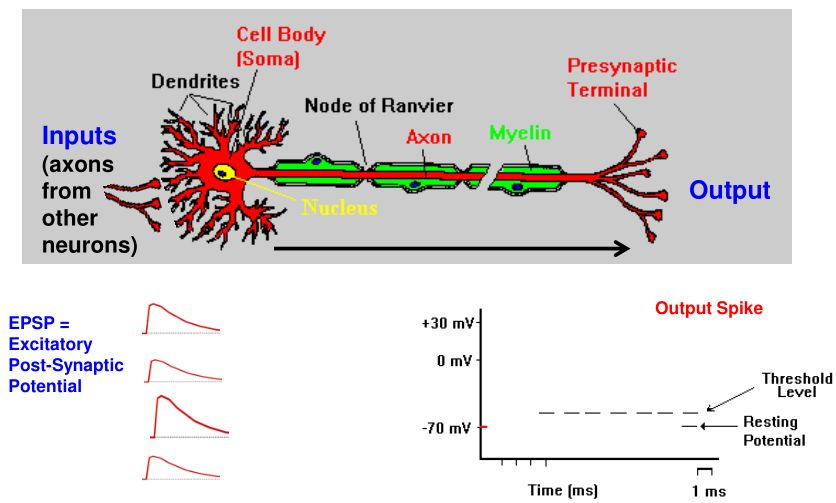
\includegraphics[width=0.9\textwidth]{idealized-neuron}
\end{figure}

\begin{figure}[H]
	\caption[What is a Neuron?]{What is a Neuron?}
	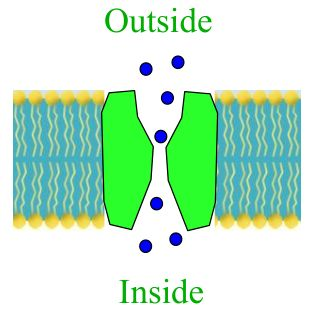
\includegraphics[width=0.9\textwidth]{what-is-a-neuron}
\end{figure}

\begin{itemize}
	\item  A “leaky bag of charged liquid”
	\item Contents of the neuron enclosed within a cell membrane
	\item Cell membrane is a lipid bilayer
	\begin{itemize}
		\item Bilayer is impermeable to charged ion species such as $Na^+$ , $Cl^-$, and $K^+$
		\item Ionic channels embedded in 	membrane allow ions to flow in or out
	\end{itemize}
\end{itemize}

\begin{figure}[H]
	\caption[The Electrical Personality of a Neuron]{The Electrical Personality of a Neuron}
	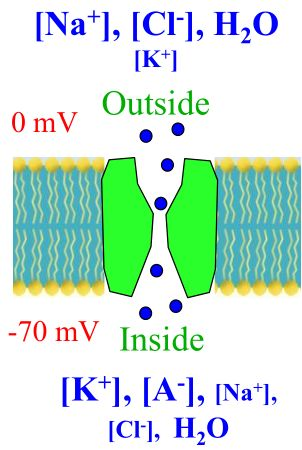
\includegraphics[width=0.9\textwidth]{what-is-a-neuron2}
\end{figure}

\begin{itemize}
	\item Each neuron maintains a potential difference across its membrane
	\item Inside is about –70 mV relative to outside
	\item $Na^+$ \& $Cl^-$ higher outside;
	$K^+$ and organic anions $A^-$	higher inside
	\item Ionic pump maintains -70 mV difference by expelling $Na^+$ out
	and allowing$K^+$ ions in
\end{itemize}

How can the electrical potential be changed in local regions of a neuron?

\begin{itemize}
	\item Ionic channels in membranes are 	proteins that are selective and
	allow only specific ions to pass 	through
	\item E.g. Pass Na + but not K + or Cl -
	\item Ionic channels are gated
	\begin{itemize}
		\item 	Voltage-gated: Probability of 	opening depends on membrane voltage
		\item Chemically-gated: Binding to a 	chemical causes channel to open
		\item Mechanically-gated: Sensitive to 	pressure or stretch
	\end{itemize}
\end{itemize}

\begin{figure}[H]
	\caption[Gated Channels allow Neuronal Signaling]{Gated Channels allow Neuronal Signaling}
	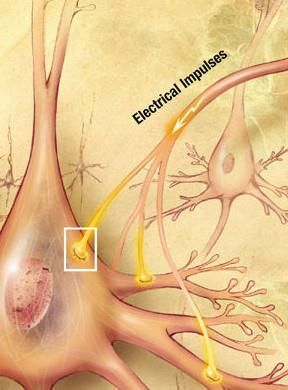
\includegraphics[width=0.9\textwidth]{signalling}
\end{figure}

\begin{itemize}
	\item Inputs from other neurons $\rightarrow$
	chemically-gated channels (at
	“synapses”) open  $\rightarrow$ Changes in
	local membrane potential
	\item This in turn causes opening/closing
	of voltage-gated channels in
	dendrites, body, and axon, resulting
	in depolarization (positive change
	in voltage) or hyperpolarization
	(negative change in voltage)
	\item Strong enough depolarization
	causes a spike or “action potential”
\end{itemize}
\begin{figure}[H]
	\caption[The Output of a Neuron: Action Potential (Spike)]{The Output of a Neuron: Action Potential (Spike). Voltage-gated channels cause action potentials (spikes) Strong depolarization opens Na + channels, causing rapid
		Na + influx and more channels to open, until they inactivate. K + outflux restores membrane potential}
	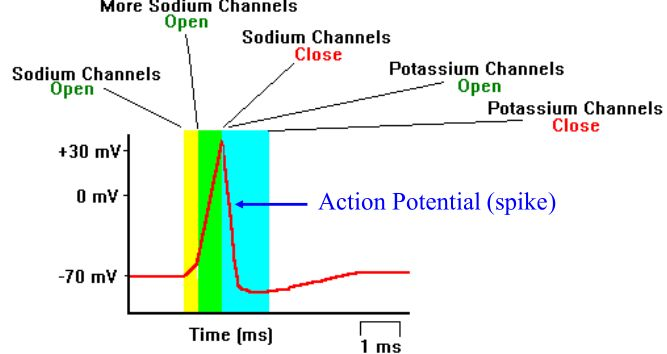
\includegraphics[width=0.9\textwidth]{action-potential}
\end{figure}

\begin{figure}[H]
	\caption[Propagation of a Spike along an Axon]{Propagation of a Spike along an Axon}
	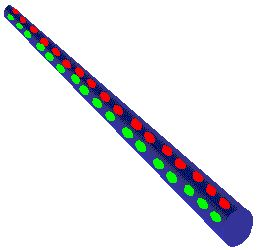
\includegraphics[width=0.9\textwidth]{propagation1}
\end{figure}

\begin{figure}[H]
	\caption[Receptive Fields: a Mechanistic Model]{Receptive Fields: a Mechanistic Model}
	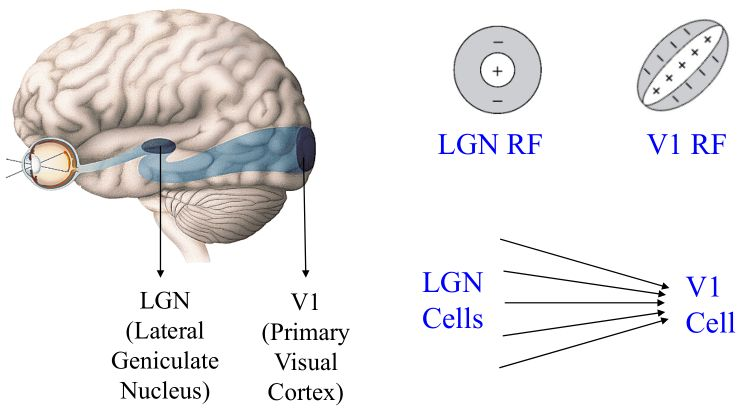
\includegraphics[width=0.9\textwidth]{mech-rf}
\end{figure}

\begin{figure}[H]
	\caption[Active Wiring: Myelination of Axons]{Active Wiring: Myelination of Axons. Myelin due to oligodendrocytes (glial cells) wrap axons and
		enable fast long-range spike communication
		Action potential “hops” from one non-myelinated region
		(node of Ranvier) to the next (saltatory conduction)
		“Active wire” allows lossless signal propagation}
	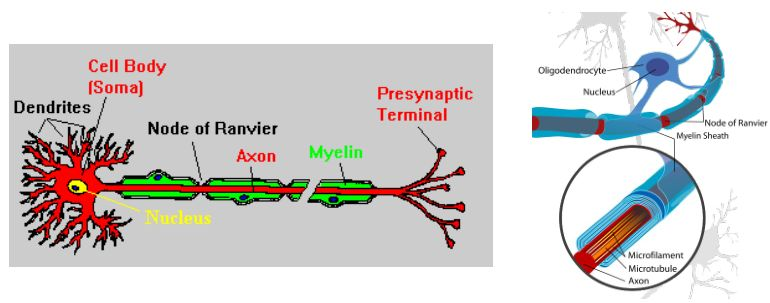
\includegraphics[width=0.9\textwidth]{myelination}
\end{figure}



\subsection{Making Connections - Synapses}
\begin{figure}[H]
	\caption[Enter the Synapse]{What happens to the spike 	(action potential) when	it reaches the 	end of an axon?	Enter the Synapse}
	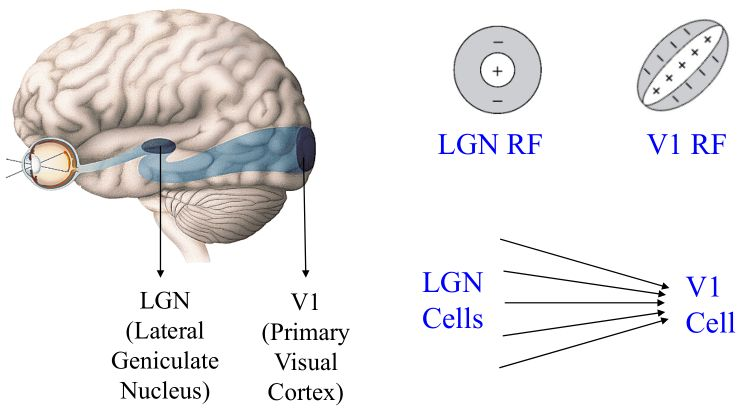
\includegraphics[width=0.9\textwidth]{mech-rf}
\end{figure}

\begin{figure}[H]
	\caption[Receptive Fields: a Mechanistic Model]{Receptive Fields: a Mechanistic Model}
	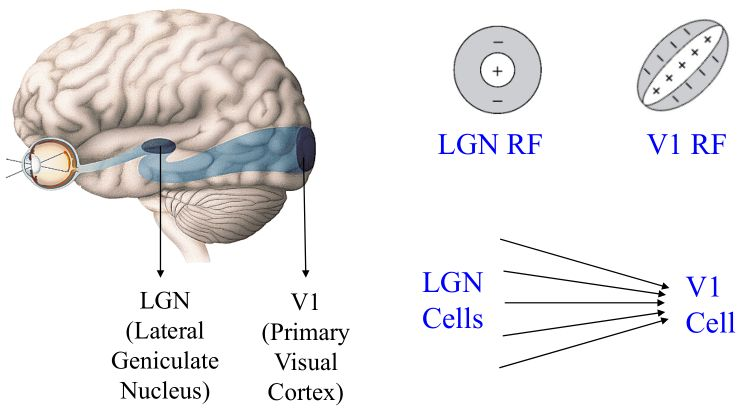
\includegraphics[width=0.9\textwidth]{mech-rf}
\end{figure}

\subsection{Time to Network - Brain Areas and their Function}

\begin{figure}[H]
	\caption{Brain Regions}
	\begin{subfigure}[b]{0.45\textwidth}
		\caption{Hind Brain. \emph{Medulla Oblongata} controls breathing, muscle tone and blood pressure.
			\emph{Pons} connected to the cerebellum \& involved in sleep and arousal.
			\emph{Cerebellum} Coordination and timing of voluntary movements, sense of equilibrium, language, attention}
		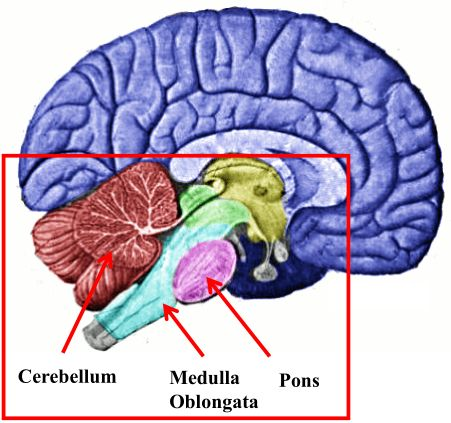
\includegraphics[width=\textwidth]{hindbrain}
	\end{subfigure}
	\begin{subfigure}[b]{0.45\textwidth}
		\caption{\emph{Midbrain} Eye movements, visual and auditory reflexes.
			\emph{Reticular Formation} 	Modulates muscle reflexes, breathing \& pain perception. Also regulates sleep, 			wakefulness \& 	arousal.}
		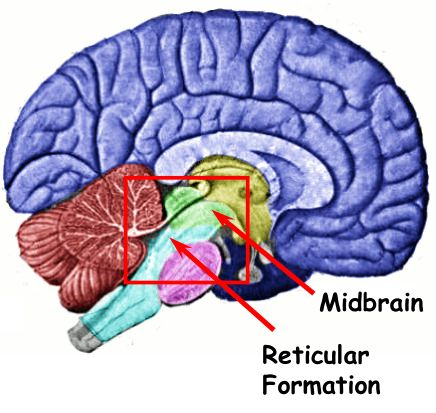
\includegraphics[width=\textwidth]{midbrain}
	\end{subfigure}
	\begin{subfigure}[b]{0.45\textwidth}
		\caption{\emph{Thalamus} Relay station for all 	sensory info (except 	smell) to the cortex, regulates sleep/wakefulness.
		\emph{Hypothalamus} Regulates basic needs: 	Fighting, Fleeing, 	Feeding, and Mating.}
		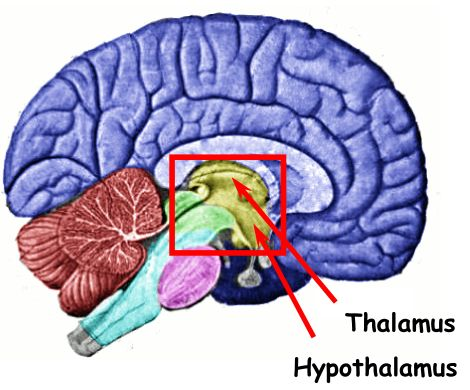
\includegraphics[width=\textwidth]{thalamus}
	\end{subfigure}
	\begin{subfigure}[b]{0.45\textwidth}
		\caption{ Consists of: Cerebral cortex, basal ganglia, 	hippocampus, and amygdala
		Involved in perception 	and motor control, 	cognitive functions,	emotion, memory, and learning}
		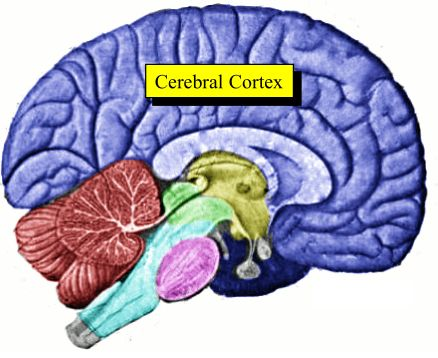
\includegraphics[width=\textwidth]{Cerebrum}
	\end{subfigure}
\end{figure}
\section{What do Neurons Encode?}\label{sec:week2}
\subsection{What is the Neural Code}
During this course, we will talk about:
\begin{itemize}
	\item techniques for recording from the brain--Figure \ref{fig:recording};
	\item  tools for discovering how the brain represents information;
	\item models that express our understanding of this representation;
	\item  some methods for inferring what the brain is doing based on its activity--Section \ref{sec:week3};
	\item  using information theory to quantify neural representations--Section \ref{sec:week4};
	\item the biophysical basis of how the brain processes inputs and performs complex computations--Section \ref{sec:week5}.
\end{itemize}

\begin{figure}[H]
	\caption[Recording from the Brain]{Recording from the Brain. (\subref{fig:rb1}) \& (\subref{fig:rb2}) \gls{gls:fMRI}: resolution $1\;mm^3$; response is averaged over many neurons, and is slow. (\subref{fig:rb3}) \gls{gls:EEG}: response is averaged over many neurons; EEG is faster than fMRI, but noisy. (\subref{fig:rb4}) \& (\subref{fig:rb5}) Electrode Arrays: good if we have access to tissue directly} \label{fig:recording} (\subref{fig:rb6} Calcium Imaging. Cells have markers that change the colour of fluorescence as calcium levels change in response to neural activity.)
	\begin{subfigure}[b]{0.3\textwidth}
		\caption{}\label{fig:rb1}
		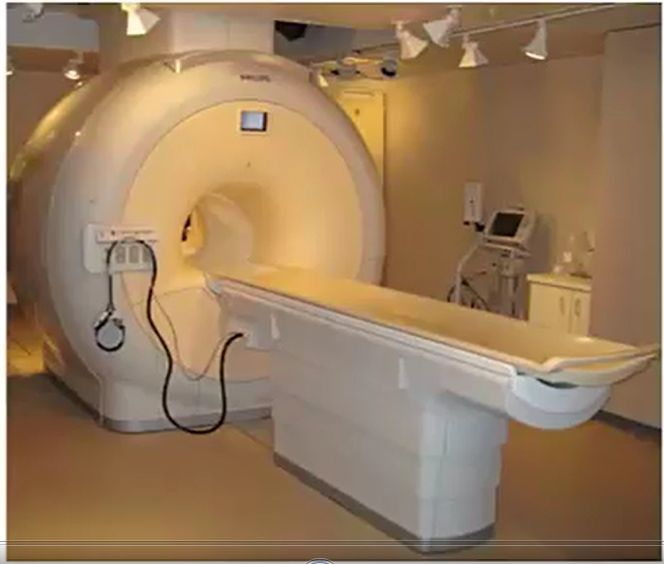
\includegraphics[width=0.9\textwidth]{fMRI}
	\end{subfigure}
	\begin{subfigure}[b]{0.3\textwidth}
		\caption{}\label{fig:rb2}
		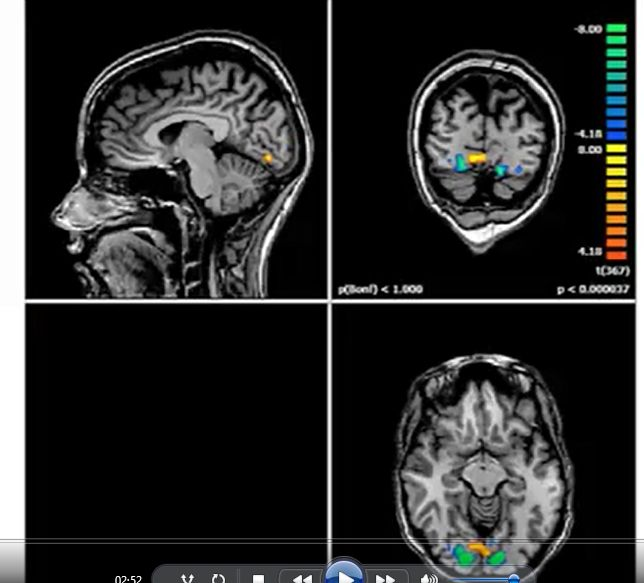
\includegraphics[width=0.9\textwidth]{fMRI2}
	\end{subfigure}
	\begin{subfigure}[b]{0.3\textwidth}
		\caption{}\label{fig:rb3}
		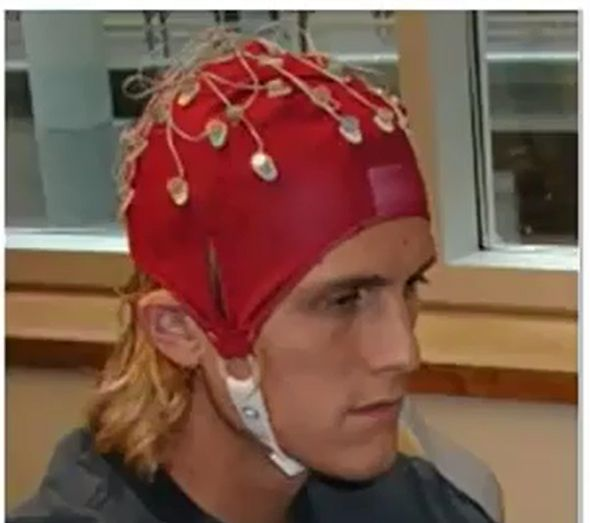
\includegraphics[width=0.9\textwidth]{EEG}
	\end{subfigure}
	\begin{subfigure}[b]{0.3\textwidth}
		\caption{}\label{fig:rb4}
		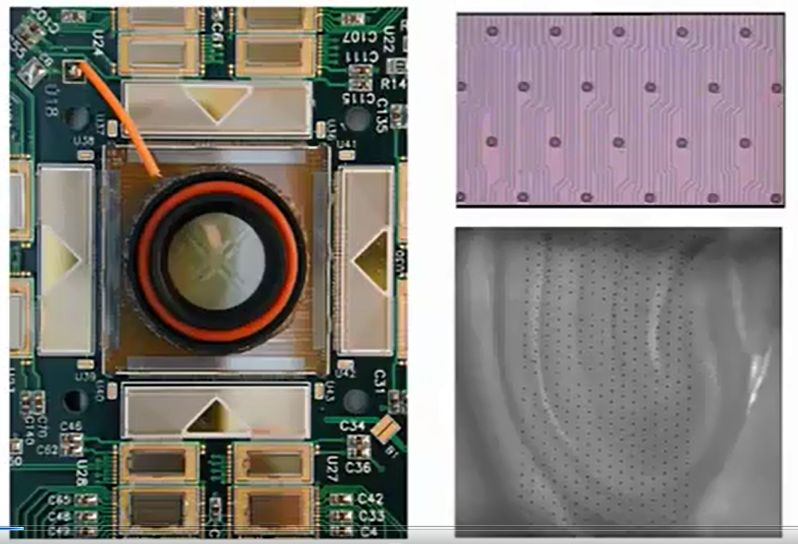
\includegraphics[width=0.9\textwidth]{electrode-arrays}
	\end{subfigure}
	\begin{subfigure}[b]{0.3\textwidth}
		\caption{}\label{fig:rb5}
		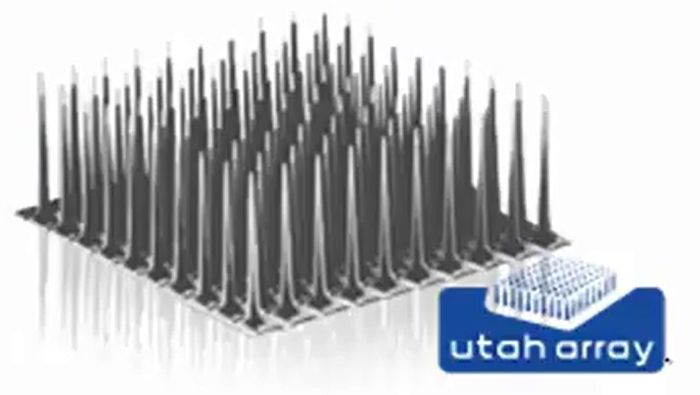
\includegraphics[width=0.9\textwidth]{electrode-arrays2}
	\end{subfigure}
	\begin{subfigure}[b]{\textwidth}
		\caption{}\label{fig:rb6}
		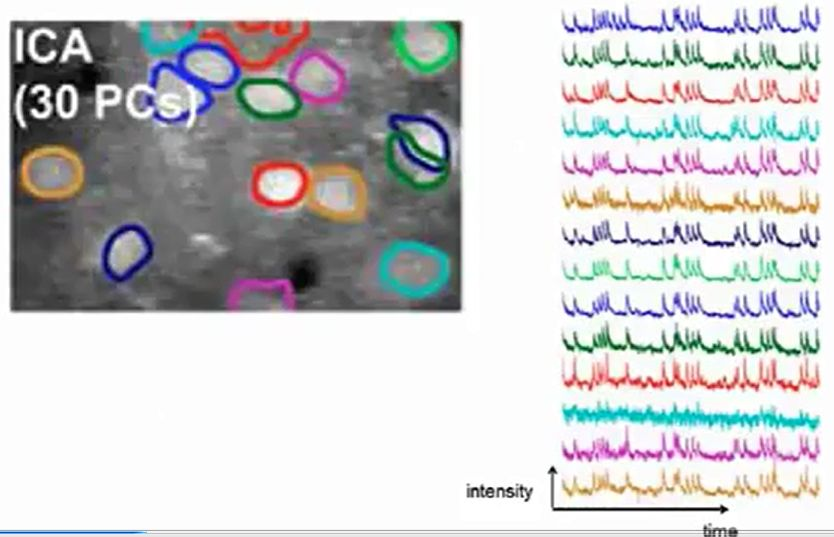
\includegraphics[width=0.9\textwidth]{calcium-imaging}
	\end{subfigure}
\end{figure}

\begin{figure}[H]
	\begin{center}
		\caption[Looking inside a single cell]{Looking inside a single cell. The experimenter clamps a patch electron onto the cell membrane}
		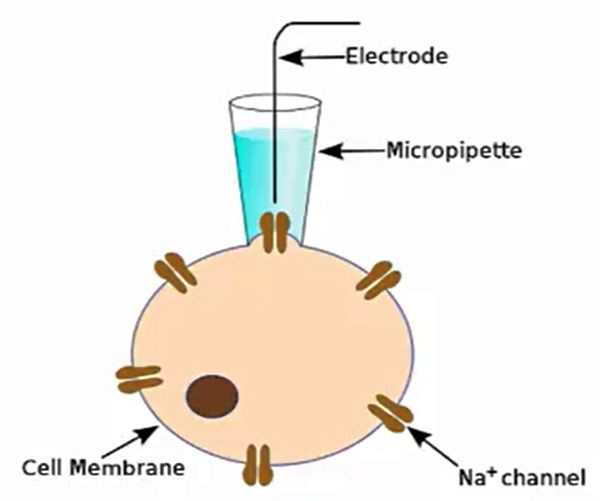
\includegraphics[width=0.9\textwidth]{looking-inside}
	\end{center}
\end{figure}

\begin{figure}[H]
	\begin{center}
		\caption{What is the neural code?}
		\begin{subfigure}[t]{0.45\textwidth}
			\caption{Human eye, without output to optic nerve}
			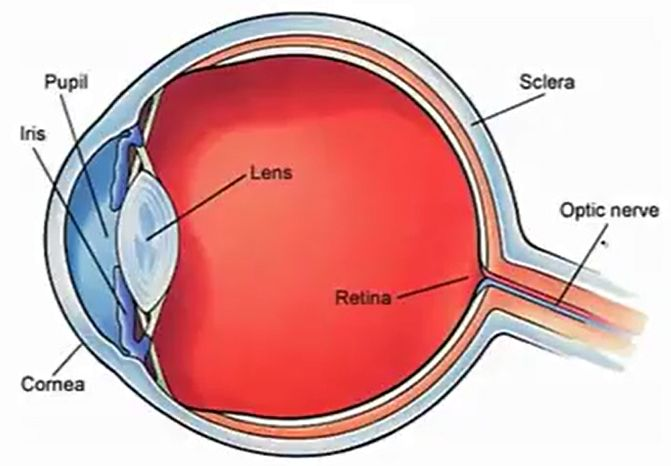
\includegraphics[width=\textwidth]{human-eye}
		\end{subfigure}
		\begin{subfigure}[to]{0.45\textwidth}
			\caption{Experiment. Play movie while section of retina is connected to electrode array--Figures \ref{fig:rb4} \& \ref{fig:rb5}}
			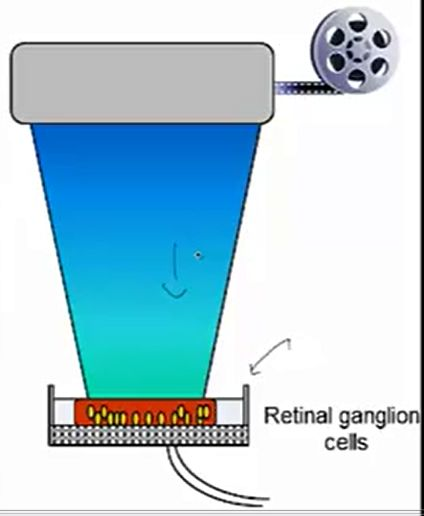
\includegraphics[width=\textwidth]{human-eye-experiment}
		\end{subfigure}
		\begin{subfigure}[to]{0.45\textwidth}
			\caption{Repeat experiment: red dots represent firings (action potentials). Notice that many times the firings are in almost the same place.}
			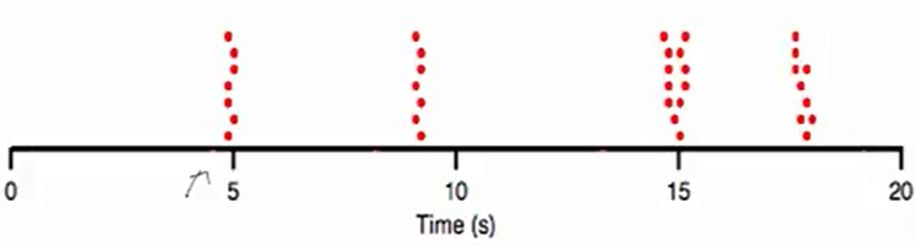
\includegraphics[width=\textwidth]{movie-firings}
		\end{subfigure}
		\begin{subfigure}[to]{0.45\textwidth}
			\caption{Look at 20 retinal ganglion cells. Each cell is reasonably consistent in time. Each cell is responsible for encoding some set of features, and different neurons encode different features. R \& P have some features in common.}\label{fig:movie-firings-20}
			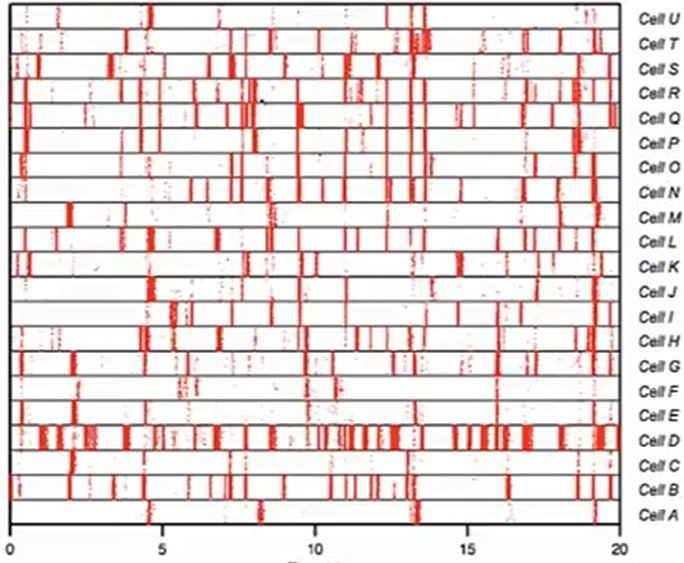
\includegraphics[width=\textwidth]{movie-firings-20}
		\end{subfigure}
	\end{center}
\end{figure}

\begin{itemize}
	\item Encoding: how does a stimulus cause a pattern of responses?
	\item\begin{itemize}
		\item  Building quasi mechanistic models
	\end{itemize}
	\item Decoding: what do these responses tell us about the stimulus?
	\item \begin{itemize}
		\item how can we reconstruct what the brain is doing?
	\end{itemize}
\end{itemize}

\begin{align*}
	P(response\vert stimulus)&\text{, encoding} \numberthis \label{eq:p_r_s}\\
	P(stimulus\vert response)&\text{, decoding}  \numberthis \label{eq:p_s_r}
\end{align*}

\begin{itemize}
	\item What is the stimulus--$s$?
	\item What is the response--$r$?
	\item what is the relation between them?
\end{itemize}
\begin{figure}[H]
	\begin{center}
		\caption[Gaussian tuning curve of a cortical (V1) neuron]{Gaussian tuning curve of a cortical (V1) neuron. These neurons respond to oriented bars.}
		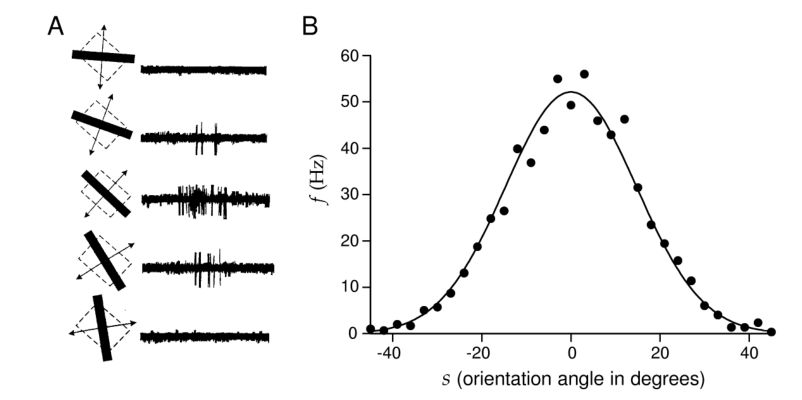
\includegraphics[width=0.9\textwidth]{tuning-curves}
	\end{center}
\end{figure}

\begin{figure}[H]
	\begin{center}
		\caption{Cosine tuning curve of a motor cortical neuron}
		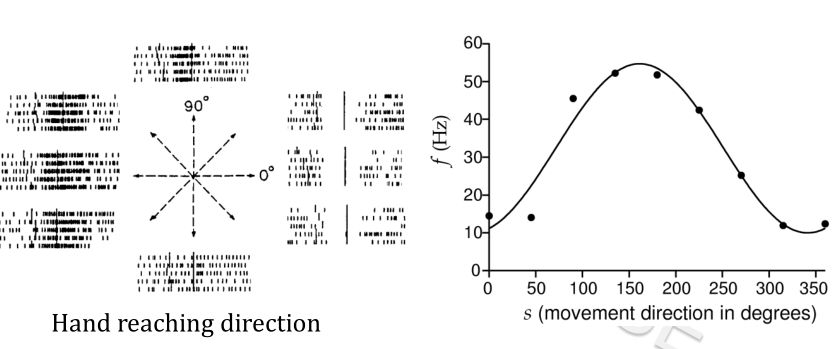
\includegraphics[width=0.9\textwidth]{tuning-curves1}
	\end{center}
\end{figure}

\begin{figure}[H]
	\begin{center}
		\caption{Feature Map in Primary Visual Cortex}
		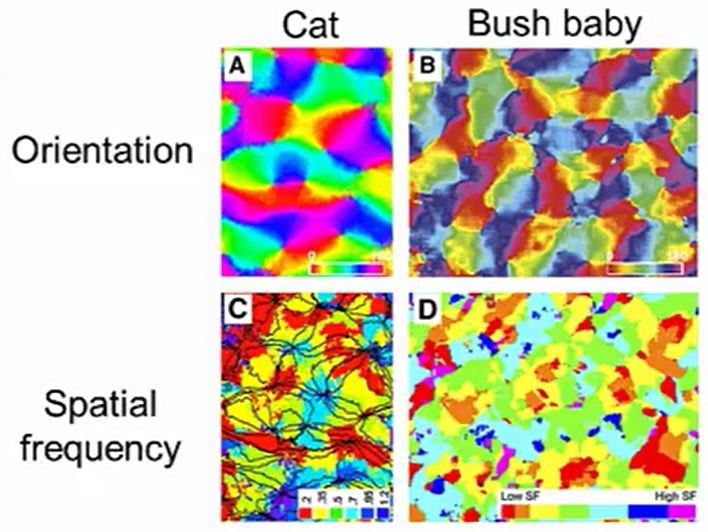
\includegraphics[width=0.9\textwidth]{feature-map}
	\end{center}
\end{figure}

\begin{figure}[H]
	\begin{center}
		\caption{Higher order features in temporal lobe}
		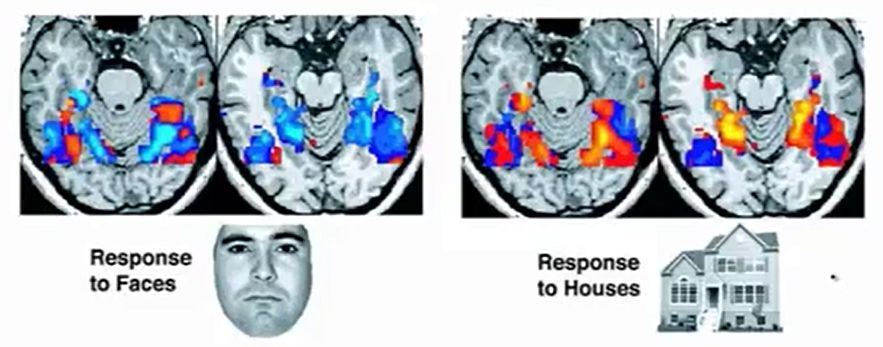
\includegraphics[width=0.9\textwidth]{higher-order-features}
	\end{center}
\end{figure}

\begin{figure}[H]
	\begin{center}
		\caption[Building up more complex features]{Building up more complex features. Notice feed-forward and feed-back.}
		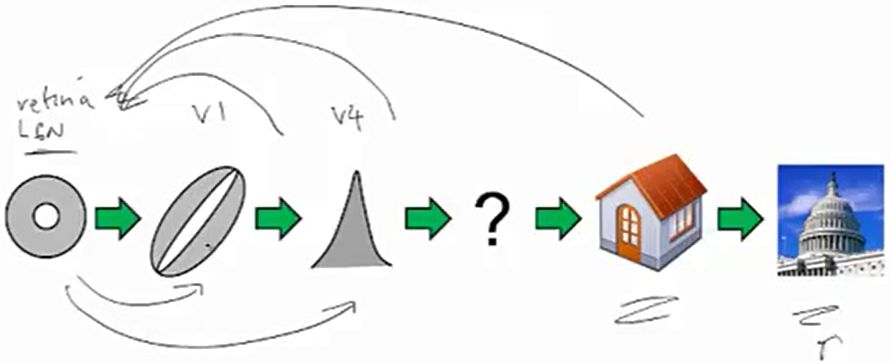
\includegraphics[width=0.9\textwidth]{build}
	\end{center}
\end{figure}

\subsection{Neural Encoding - Simple Models}

We  consider the case where a response is a single spike. We want to determine $P(R\vert S) \rightarrow r(t)$, where $r(t)$ is the firing rate, given a stimulus $s$.

\begin{figure}[H]
	\begin{center}
		\caption{Simplest possible model: $r(t) = \phi s(t-\tau)$)}
		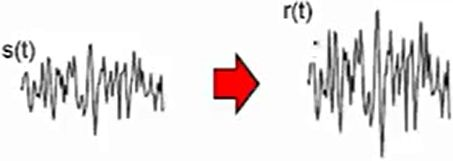
\includegraphics[width=0.9\textwidth]{simplest-model}
	\end{center}
\end{figure}

\subsubsection{What about a linear filter?}

\begin{align*}
	r(t) =& \sum_{i=1}^{n} s_{t-i} f_i \text{, or spatial filtering} \numberthis \label{eq:linear:filter}\\
	r(x,y) =& \sum_{x^\prime=-n,y^\prime=-n}^{n,n}s_{x-x^\prime,y-y^\prime} f_{x^\prime,y^\prime} \text{, as in Figure \ref{fig:rf1}}
\end{align*}

\begin{figure}[H]
	\begin{center}
		\caption[Receptive Field]{Receptive Field: (\subref{fig:rf1}) is a cartoon view, (\subref{fig:rf2}) shows the filter as a difference between two Gaussians; (\subref{fig:rf4}) shows the effect of applying the filter to (\subref{fig:rf3}.)}
		\begin{subfigure}[t]{0.45\textwidth}
			\caption{Cartoon}\label{fig:rf1}
			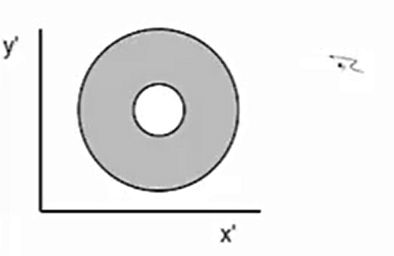
\includegraphics[width=0.9\textwidth]{receptive-field1}
		\end{subfigure}
		\begin{subfigure}[t]{0.45\textwidth}
			\caption{Detailed view}\label{fig:rf2}
			\includegraphics[width=0.9\textwidth]{receptive-field2}
		\end{subfigure}
		\begin{subfigure}[t]{0.45\textwidth}
			\caption{Taj Mahal}\label{fig:rf3}
			\includegraphics[width=0.9\textwidth]{receptive-field3}
		\end{subfigure}
		\begin{subfigure}[t]{0.45\textwidth}
			\caption{Filtered Taj Mahal, showing edges only}\label{fig:rf4}
			\includegraphics[width=0.9\textwidth]{receptive-field4}
		\end{subfigure}
	\end{center}
\end{figure}

\begin{figure}[H]
	\caption[Spatiotemporal filtering]{Spatiotemporal filtering. $r_{x,y}(t)=\int dx^\prime dy^\prime d\tau f(x^\prime,y^\prime,\tau) s((x-x^\prime,y-y^\prime,t-\tau)$}
	\includegraphics[width=0.9\textwidth]{spatio--temporal-filtering}
\end{figure}

\subsubsection{Linear filters cannot be the full picture}

Linear filters have a few limitations:
\begin{itemize}
	\item they can give rise to a negative firing rate!
	\item they can increase indefinitely!
\end{itemize} 

We need to impose a non-linearity, so \eqref{eq:linear:filter} becomes:
\begin{align*}
	r(t) =& g\big(\sum_{i=1}^{n} s_{t-i} f_i\big) \numberthis \label{eq:non-linearity}
\end{align*}

\begin{figure}[H]
	\caption{Filter showing effect of saturating non-linearity}
	\includegraphics[width=0.9\textwidth]{saturated}
\end{figure}

\subsection{Neural Encoding - Feature Selection}
How to find the components of \eqref{eq:non-linearity}? Our problem is dimensionality! We want to sample the responses of the system to many stimuli, so we can characterize what it is about the input that drives responses. We will start with a very high dimensional description and pick out a small set of relevant dimensions.

\begin{figure}[H]
	\caption[Dimensionality Reduction]{Dimensionality Reduction: $P(response|stimulus)\rightarrow P(response\vert s_1,s_2,...s_n)$}
	\includegraphics[width=0.9\textwidth]{dimenionality-reduction}
\end{figure}

Gaussian white noise is a useful method.

\begin{figure}[H]
	\caption[Determining multiple features from white noise]{Determining multiple features from white noise. This allows us to create a Gaussian prior. This will be a multivariate Gaussian, no matter which axes we use.}\label{fig:determining-multiple-features}
	\includegraphics[width=0.9\textwidth]{white-noise}
\end{figure}

\begin{figure}[H]
	\caption[Spike Conditioned Distribution]{Spike Conditioned Distribution. We project onto a vector representing mean of spike-conditioned points}\label{fig:spike:conditioned}
	\includegraphics[width=0.9\textwidth]{spike-conditioned-distribution}
\end{figure}

\begin{figure}[H]
	\caption[Reverse Correlation: the spike triggered average]{Reverse Correlation: the spike triggered average. Every time there is a spike, grab the portion of signal that preceded it, forming an ensemble, which we average. This represents what is common to stimuli that triggered response.}
	\includegraphics[width=0.9\textwidth]{reverse-correlation}
\end{figure}

\begin{figure}[H]
	\caption[Spike Triggered average for vector]{Spike Triggered average for vector, maybe in image that has been turned into a single vector}
	\includegraphics[width=0.9\textwidth]{sta-image}
\end{figure}

In each of these cases we have a vector that represents a feature, and we project the stimulus onto this unit vector. How do we compute the input-output curve, the function $g$ from \eqref{eq:non-linearity}? 

\begin{align*}
	P(spike\vert stimulus) \rightarrow& P(spike\vert s_1) \text{. This can be found using Bayes' rule.}\\
	 P(spike\vert s_1) =& \frac{\overbrace{P(s_1\vert spike)}^\text{Factor from Figure \ref{fig:factors:bayes}} \cdot \overbrace{P(spike)}^\text{Prior from Figure \ref{fig:determining-multiple-features}}}{\underbrace{P(s_1)}_\text{Factor from Figure \ref{fig:factors:bayes}}}
\end{align*}


\begin{figure}[H]
	\caption[Factors used in Bayes Rule]{Factors used in Bayes Rule}\label{fig:factors:bayes}
	\includegraphics[width=0.9\textwidth]{compondents-of bayes}
\end{figure}


\begin{figure}[H]
	\caption[Examples of IO curves]{Examples of IO curves. The left hand curve shows no impact from the stimulus; either there is none, or we have chosen the wrong vector.}\label{fig:sample-io-curves}
	\includegraphics[width=0.9\textwidth]{sample-io-curves}
\end{figure}

\subsubsection{High-dimensional Feature Selection}

We select some subset of features that are relevant to a decision: $r(t)=g(f_1*s, f_2*x,...)$. How can we extract more information from Figure \ref{fig:spike:conditioned}?

\begin{figure}[H]
	\caption[High-dimensional Feature Selection]{High-dimensional Feature Selection. We could extract higher order moments, or the covariance. Can use PCA to reduce dimensionality.}
	\includegraphics[width=0.9\textwidth]{spike-conditioned-distribution-covariance}
\end{figure}

\begin{figure}[H]
	\caption[Most faces can be reconstructed from a set of 7-8 eigenfaces]{Although it takes a lot of pixels to represent a face, there is a lot structure, and most faces can be reconstructed from a set of 7-8 principle components, known as ``eigenfaces''.}
	\includegraphics[width=0.9\textwidth]{eigenfaces}
\end{figure}

\begin{figure}[H]
	\caption[Use of PCA to sort out spikes]{Use of PCA to sort out spikes from two or more neurons recorded from a single electrode}
	\includegraphics[width=0.9\textwidth]{pca-spike-sorting}
\end{figure}

\begin{figure}[H]
	\caption[Finding Interesting Features in the Retina using PCA]{Finding Interesting Features in the Retina using PCA. Each blue dot represents 100 steps of a white-noise flicker. Spike triggered average is zero: we have two features, one which recognizes light turning on, the other off.}
	\includegraphics[width=0.9\textwidth]{finding-interestimg-features}
\end{figure}

\subsection{Neural Encoding - Variability}

There are a couple of things in Figure \ref{fig:movie-firings-20} that we still need to address: we modeled only a time varying firing rate, so thee are hidden assumptions about the rates at which signals and responses vary. There appears to be some fins structure that we have missed.

When have you found a good feature or features?
\begin{itemize}
	\item When the input/output curve over your variable is interesting
	\item How to quantify interesting?
\end{itemize}

\subsubsection{Quantifying Interesting}
In Figure \ref{fig:sample-io-curves}, the left hand curve is boring, the right interesting. Can we exploit the tuning curve and find a $f$ that maximizes the difference between the prior and posterior?

\begin{align*}
	P(spike\vert s_f) =&\frac{ P(s_f\vert spike) P_({spike})}{P(s_f)}
\end{align*}
 We introduce the Kullback-Leibler divergence
\begin{align*}
		D_{KL}(P(s),Q(s))\triangleq&\mathbb{E}_{P(s)} \Big(\log_2 \frac{P(s)}{Q(s)}\Big) \text{, and maximize}\\
		D_{KL}(P(s_f|spike),P(s_f))
\end{align*}

\begin{figure}[H]
	\caption[Maximally Informative Dimensions]{Maximally Informative Dimensions: choose filter to maximize $K_{DL}$ between spike-conditioned and prior distributions. This turns out to be equivalent to maximizing mutual information-\eqref{eq:mutual:information}. Notice that the stimulus is not necessarily Gaussian.}
	\includegraphics[width=0.9\textwidth]{maximally-informative-dimensions}
\end{figure}
This technique:
\begin{itemize}
	\item does not depend on white noise inputs;
	\item can be used for deriving models from natural stimuli;
	\item but is not guaranteed to give rise to a unique maximum.
\end{itemize}

Summary--finding relevant features:
\begin{enumerate}
	\item single filter determined by the conditional average;
	\item  a family of filters derived using PCA;
	\item information theoretic methods use the whole distribution.
\end{enumerate}

\subsubsection{Modelling the noise}

We can model spikes that may or may not occur with a series of time bins, each of which may or may not contain a spike. In the limit where there are many bons we can use the Poisson distribution.

\begin{align*}
	P_T(k) =& (rT)^k\frac{\exp(-rT)}{k!}\\
	<k> =& rT\\
	var(k) =& rT\\
	F =& 1 \text{, Fano factor}\\
	P(T)=&r \exp(-rT)
\end{align*}

\begin{figure}[H]
	\caption[Poisson or not?]{Poisson or not? Monkey is watching a movie. Rate is variable. Split time into bins and plot mean number of spikes and variance in each bin. Firing rate changes, but Fano remains close to 1.}
	\includegraphics[width=0.9\textwidth]{poisson-or-not}
\end{figure}

\begin{figure}[H]
	\caption[Interspike Interval Distributions]{Interspike Interval Distributions. A typical cortical neuron is connected to 10,000 others: average input may be zero, but there will be some jitter. Right hand image zooms in on short intervals, which are no longer Poisson for a good reason: a neuron's firing rate is limited by physics.}
	\includegraphics[width=0.9\textwidth]{interspike-intervals}
\end{figure}

\begin{figure}[H]
	\caption[Generalized Linear Model]{Generalized Linear Model\cite{pillow2008spatio}. $P(spike\;at\;t) \propto \exp(f_1*s + h_1*r)$. The exponential nonlinearity allows all parameters to be determined using an optimization scheme that is globally convergent.}
	\includegraphics[width=0.9\textwidth]{generalized-linear-model}
\end{figure}

\begin{figure}[H]
	\caption[Coupled Spiking Model]{Coupled Spiking Model\cite{pillow2008spatio}. $P(spike\;at\;t) \propto \exp(f_1*s + h_1*r_1+h_2*r_2)$.}
	\includegraphics[width=0.9\textwidth]{coupled-spiking-model}
\end{figure}

\begin{figure}[H]
	\caption[Time Rescaling Theorem]{The Time Rescaling Theorem\cite{brown2002time} allows us to determine whether we have captured everything we can from the inputs to out model. Scale output time intervals by firing rate that model predicted. If predicted rate accounts for all the influences on the firing, then scaled intervals should be distributed like a pure Poisson process with an effective rate of 1.} 
	\includegraphics[width=0.9\textwidth]{time-rescaling-thorem}
\end{figure}

\section{Extracting Information from Neurons}\label{sec:week3}

\subsection{Neural Decoding and Signal Detection Theory}

\begin{figure}[H]
		\caption[Value of threshold that maximizes probability of correct call]{This value of threshold maximizes probability of calling correctly.
			$p[+]p[r\ge z\vert +] + p[-] (1-p[r\ge z\vert -])$}
		\includegraphics[width=\textwidth]{signal-detection1}
\end{figure}
\subsection{Population Coding and Bayesian Estimating}

\begin{align*}
	\underbrace{p[s\vert r]}_\text{A posteriori distribution} =& \frac{\overbrace{p[r\vert s]}^\text{Likelihood function} \cdot \overbrace{p[s]}^\text{Prior distribution}}{\underbrace{p[r]}_\text{Marginal distribution}} \text{, where}\\
	p[r] =& \int ds \; p[r\vert s] p[s]
\end{align*}

\begin{itemize}
	\item \gls{gls:ML} \gls{gls:mlm}
	\item \gls{gls:MAP} \gls{gls:mpm}
\end{itemize}
 An example. Assume:
 
\begin{enumerate}
	\item a population of neurons that encode some stimulus $s$
	\item response is Gaussian (e.g. V1)
	\item each fires independently
	\item Poisson Firing\label{item:poisson}
\end{enumerate}

\begin{figure}[H]
	\caption{Gaussian Tuning Curves}
	\includegraphics[width=\textwidth]{decode-stimulus}
\end{figure}

\begin{align*}
	f_a(s) =& r_{max} \exp \Big(-\frac{1}{2}\big[\frac{s-s_a}{\sigma_a}\big]^2\Big)\text{, assume good coverage} \numberthis \label{eq:gauss}\\
	\sum_{1}^{N} f_a(s) =& const \numberthis \label{eq:good:coverage}
\end{align*}

So firing rate doesn't depend on stimulus

From assumption \ref{item:poisson}, spikes are produced randomly and independently in each time bin with probability
\begin{align*}
	P_T[k] =& \frac{(rT)^k \exp (-rT)}{k!}\\
	P_T[r_a\vert s] =& \frac{(f_a(s)T)^{r_aT} \exp (-f_a(s)T)}{r_aT!}\\
	P[\vec{r}\vert s] =& \prod_{a=1}^{N}P_r[a\vert s]\\
	=& \prod_{a=1}^{N} \frac{(f_a(s)T)^{r_aT} \exp (-f_a(s)T)}{r_aT!}
\end{align*}

We want the \gls{gls:ML} for $s$.
\begin{align*}
	\ln P[\vec{r}\vert s] =& \sum_{a=1}^{N} \big[r_aT \ln (f_a(s)T) -f_a(s)T - \ln (r_aT!) \big] \text{, so we need}\\
	\nabla_a \ln P[\vec{r}\vert s] =& 0	
\end{align*}
 where  $\nabla_a$ denotes the operator $\frac{\partial}{\partial_{s_a}}$. Now
\begin{align*}
	\nabla_a \ln P[\vec{r}\vert s] = & \partial_a \sum_{a=1}^{N}  r_aT \ln (f_a(s)T) -\underbrace{\partial_a \sum_{a=1}^{N} f_a(s)T}_{=0 \text { from ]\eqref{eq:good:coverage}}} - \underbrace{\partial_a \sum_{a=1}^{N} \ln (r_aT!)}_{=0} 
\end{align*}
Hence the \gls{gls:mlm} is given by:
\begin{align*}
	T \partial_a \sum_{a=1}^{N} r_a  \ln (f_a(s)T) =& 0\\
	 \sum_{a=1}^{N} r_a  \partial_a \ln (f_a(s)T) =& 0\\
	 \sum_{a=1}^{N} r_a  \frac{\partial_a  (f_a(s)\cancel{T})}{(f_a(s)\cancel{T})} =& 0\\
	 \sum_{a=1}^{N} r_a  \frac{\partial_a  f_a(s^*)}{f_a(s^*)} =& 0 \numberthis \label{eq:ml:example}
\end{align*}

\begin{align*}
	\partial_a  f_a(s) =& \partial_a r_{max} \exp \Big(-\frac{1}{2}\big[\frac{s-s_a}{\sigma_a}\big]^2\Big)\\
	=&r_{max}\big[-\frac{1}{\cancel{2}} \frac{\cancel{2}(s-s_a)}{\sigma_a^2}\big] \exp \Big(-\frac{1}{2}\big[\frac{s-s_a}{\sigma_a}\big]^2\Big)\\
	=& \frac{\cancel{2}(s-s_a)}{\sigma_a^2} f_a(s) \text{, so \eqref{eq:ml:example} becomes}
\end{align*}
\begin{align*}
	\sum_{a=1}^{N} r_a  \frac{(s^*-s_a)}{\sigma_a^2} =& 0\\
	s^*  =& \frac{\sum_{a=1}^{N}   \frac{s_a r_a}{\sigma_a^2}}{\sum_{a=1}^{N} \frac{ r_a }{\sigma_a^2}}	\\
	=& \frac{\sum_{a=1}^{N}   p_a s_a r_a}{\sum_{a=1}^{N} p_a r_a} \text{, where the precision $p_a=\sigma_a^{-2}$}\\
	=& \frac{\sum_{a=1}^{N}   s_a r_a}{\sum_{a=1}^{N} r_a} \text{, if all the $s_a$ are equal}
\end{align*}

For the \gls{gls:MAP} estimate, Bayes rule gives:
\begin{align*}
	\ln p[s|r] =& \ln p[r|s] + \ln p[s] - \ln p[r]\\
	=& T \sum_{a=1}^{N}r_a \ln f_a(s) + \ln p[s] + C \text{, where $C$ does not depend on $s_a$}
\end{align*}

So the \gls{gls:MAP} estimator satisfies:
\begin{align*}
	\sum_{a=1}^{N} r_a \frac{f^\prime(a^*)}{f(a^*)} + \frac{p^\prime(s)}{p(s)}=&0\\
	s^*  =& \frac{\sum_{a=1}^{N}   \frac{s_a r_a}{\sigma_a^2}+\frac{s_{prior}}{\sigma_{prior}^2}}{\sum_{a=1}^{N} \frac{ r_a }{\sigma_a^2}+\frac{1}{\sigma_{prior}^2}}
\end{align*}
\subsection{Reading Minds - Stimulus Reconstruction}
We want an estimator, $S_{Bayes}$ that gives the "best" estimate of $s$ given $r$.

\section{Entropy \& Spike Trains}\label{sec:week4}

\subsection{Information \& Entropy}

Entropy measures surprise.
\begin{align*}
	H =& - \sum_{i} p_i \log_2 p_i
\end{align*}

\begin{figure}[H]
	\begin{center}
		\caption{How about the stimulus?}
		\includegraphics[width=0.8\textwidth]{how}\label{fig:how:about:the:stimulus}
	\end{center}
\end{figure}

In Figure \ref{fig:how:about:the:stimulus}, suppose the probability of error is a constant.
\begin{align*}
	P[r_-\vert +] =& q\\
	P[r_+\vert +] =& 1-q\\
	P[r_+\vert -] =& q\\
	P[r_-\vert -] =& 1-q
\end{align*}
\begin{align*}
	H[R] =& -P[r_+] \log P[r_+] - P[r_-] \log P[r_-] \text{, total entropy}\\
	H[R\vert +] =& -q \log q - (1-q) \log (1-q) \text{, noise entropy}
\end{align*}


Mutual Information: total entropy - average noise entropy.

\begin{align*}
	I(R,S) =& -\sum_r p[r] \log p[r] - \sum_s p(s)\big[- \sum_r p[r \vert s] \log p[r \vert s]\big]\\
	=& H[R] - \sum_s p(s) H[R\vert s] \numberthis \label{eq:mutual:information}\\
\end{align*}
\begin{align*}
	I[S,R] \triangleq D_{KL}&\big[P(R,S),P(R)P(S)\big]\\
	=&H[R]-\sum_s P(s) H[R\vert s]
\end{align*}

\subsection{Calculating Information in Spike Trains}

What information is carried by patterns of spikes?

Mutual  information  is  the  difference  between  
the  total  response  entropy  and   the  mean  noise  entropy.
\begin{align*}
	I(S;R) =& H[R] - \sum_s P[s] H[R\vert s]
\end{align*}
\begin{figure}[H]
	\begin{center}
			\caption[Calculating Information in Spike Patterns]{Calculating Information in Spike Patterns. Divide into words of length $T$, e.g. $w_1=[1,0,1,0,1,1,0]$. Information is difference between total variability driven by stimuli and that dues to noise, averaged over stimuli.\cite{strong1998entropy}}
		\includegraphics[width=\textwidth]{calculatingInformationInSpikePatterns}
	\end{center}
\end{figure}

\begin{figure}[H]
	\begin{center}
		\caption[Entropy for chunked words]{Entropy for chunked words. The most common pattern is all zeroes, then a single bit, etc. nformation  :   
			difference  between  the  total  
			variability   driven  by  stimuli  
			and  that  due  to   noise,  averaged  
			over  stimuli. \cite{strong1998entropy,reinagel2000temporal}}
		\includegraphics[width=\textwidth]{info-spike-trains}
	\end{center}
\end{figure}
\subsection{Coding Principles}
\begin{itemize}
	\item What are the challenges posed by natural stimuli?
	\item What do information theoretic concepts suggest that neural systems should do?
	\item What principle seems to be at work shaping the neuarl code?
\end{itemize}

Photo - have to change F-stop repeatedly in order to capture details of scene inside and outside; the eye does this effortlessly. Natural stimuli:
\begin{enumerate}
	\item Have a wide dynamic range: variations over many orders of magnitude;
	\item dynamic scaling.
\end{enumerate}

\begin{figure}[H]
	\begin{center}
		\caption[Power Law]{Power Law: there are similar structures at very different length scales.}
		\begin{subfigure}[b]{0.45\textwidth}
			\caption{Structures}
			\includegraphics[width=0.9\textwidth]{power-law-graph}
		\end{subfigure}
		\begin{subfigure}[b]{0.45\textwidth}
			\caption{Power Spectrum: there is no characteristic scale for image.}
			\includegraphics[width=0.9\textwidth]{power-law-shapes}
		\end{subfigure}
	\end{center}
\end{figure}

\begin{figure}[H]
	\begin{center}
		\caption[Efficient Coding]{Efficient Coding: In order to have maximum entropy output, a good encoder should match its outputs to the distribution of its inputs. Try to use all symbols equally often. (cumulative probability)}
		\includegraphics[width=0.8\textwidth]{efficient-coding}
	\end{center}
\end{figure}

Contrast varies widely in time. Should neural system optimize locally or over evolutionary time?

\begin{figure}[H]
	\begin{center}
		\caption{What have we left out}
		\includegraphics[width=0.8\textwidth]{4-big-picture}
	\end{center}
\end{figure}

Make sure we have covered
\begin{enumerate}
	\item Efficient coding
	\item Sparse Coding
\end{enumerate}

\begin{align*}
	I(\vec{x}) =& \sum_{i}a_i \phi_i(\vec{x}) + \epsilon(\vec{x})\\
	E =& \mathlarger \sum_{\vec{x}}\big[I(\vec{x})-\sum_{i}a_i \phi_i(\vec{x})\big]^2 + \lambda \sum_{i}C(a_i)
\end{align*}


\section{Computing in Carbon}\label{sec:week5}

\subsection{Modeling Neurons}
TBP

\subsection{Spikes}
TBP

\subsection{Simplified Model Neurons}
TBP

\subsection{A Forest of Dendrites}
TBP

\section{Computing with Networks}\label{sec:week6}

\subsection{Making Connections between Neurons}
TBP

\subsection{Introduction to Network Models}
TBP

\subsection{Recurrent Networks}
TBP

\section{Networks that Learn}\label{sec:week7}

\subsection{Synaptic Plasticity, Hebb's Rule, and Statistical Learning}
TBP

\subsection{Introduction to Unsupervised Learning}
TBP

\subsection{Sparse Coding \& Predictive Coding}
TBP

\section{Learning from Supervision \& Rewards}\label{sec:week8}

\subsection{Neurons as Classifiers and Supervised Learning}
TBP

\subsection{Reinforcement Learning: Predicting Rewards}
TBP

\subsection{Reinforcement Learning: Time for Action!}
TBP

\appendix

\printglossaries

% bibliography goes here

\bibliographystyle{unsrt}
\addcontentsline{toc}{section}{Bibliography}
\bibliography{cns}

\end{document}
